\documentclass[1p]{elsarticle_modified}
%\bibliographystyle{elsarticle-num}

%\usepackage[colorlinks]{hyperref}
%\usepackage{abbrmath_seonhwa} %\Abb, \Ascr, \Acal ,\Abf, \Afrak
\usepackage{amsfonts}
\usepackage{amssymb}
\usepackage{amsmath}
\usepackage{amsthm}
\usepackage{scalefnt}
\usepackage{amsbsy}
\usepackage{kotex}
\usepackage{caption}
\usepackage{subfig}
\usepackage{color}
\usepackage{graphicx}
\usepackage{xcolor} %% white, black, red, green, blue, cyan, magenta, yellow
\usepackage{float}
\usepackage{setspace}
\usepackage{hyperref}

\usepackage{tikz}
\usetikzlibrary{arrows}

\usepackage{multirow}
\usepackage{array} % fixed length table
\usepackage{hhline}

%%%%%%%%%%%%%%%%%%%%%
\makeatletter
\renewcommand*\env@matrix[1][\arraystretch]{%
	\edef\arraystretch{#1}%
	\hskip -\arraycolsep
	\let\@ifnextchar\new@ifnextchar
	\array{*\c@MaxMatrixCols c}}
\makeatother %https://tex.stackexchange.com/questions/14071/how-can-i-increase-the-line-spacing-in-a-matrix
%%%%%%%%%%%%%%%

\usepackage[normalem]{ulem}

\newcommand{\msout}[1]{\ifmmode\text{\sout{\ensuremath{#1}}}\else\sout{#1}\fi}
%SOURCE: \msout is \stkout macro in https://tex.stackexchange.com/questions/20609/strikeout-in-math-mode

\newcommand{\cancel}[1]{
	\ifmmode
	{\color{red}\msout{#1}}
	\else
	{\color{red}\sout{#1}}
	\fi
}

\newcommand{\add}[1]{
	{\color{blue}\uwave{#1}}
}

\newcommand{\replace}[2]{
	\ifmmode
	{\color{red}\msout{#1}}{\color{blue}\uwave{#2}}
	\else
	{\color{red}\sout{#1}}{\color{blue}\uwave{#2}}
	\fi
}

\newcommand{\Sol}{\mathcal{S}} %segment
\newcommand{\D}{D} %diagram
\newcommand{\A}{\mathcal{A}} %arc


%%%%%%%%%%%%%%%%%%%%%%%%%%%%%5 test

\def\sl{\operatorname{\textup{SL}}(2,\Cbb)}
\def\psl{\operatorname{\textup{PSL}}(2,\Cbb)}
\def\quan{\mkern 1mu \triangleright \mkern 1mu}

\theoremstyle{definition}
\newtheorem{thm}{Theorem}[section]
\newtheorem{prop}[thm]{Proposition}
\newtheorem{lem}[thm]{Lemma}
\newtheorem{ques}[thm]{Question}
\newtheorem{cor}[thm]{Corollary}
\newtheorem{defn}[thm]{Definition}
\newtheorem{exam}[thm]{Example}
\newtheorem{rmk}[thm]{Remark}
\newtheorem{alg}[thm]{Algorithm}

\newcommand{\I}{\sqrt{-1}}
\begin{document}

%\begin{frontmatter}
%
%\title{Boundary parabolic representations of knots up to 8 crossings}
%
%%% Group authors per affiliation:
%\author{Yunhi Cho} 
%\address{Department of Mathematics, University of Seoul, Seoul, Korea}
%\ead{yhcho@uos.ac.kr}
%
%
%\author{Seonhwa Kim} %\fnref{s_kim}}
%\address{Center for Geometry and Physics, Institute for Basic Science, Pohang, 37673, Korea}
%\ead{ryeona17@ibs.re.kr}
%
%\author{Hyuk Kim}
%\address{Department of Mathematical Sciences, Seoul National University, Seoul 08826, Korea}
%\ead{hyukkim@snu.ac.kr}
%
%\author{Seokbeom Yoon}
%\address{Department of Mathematical Sciences, Seoul National University, Seoul, 08826,  Korea}
%\ead{sbyoon15@snu.ac.kr}
%
%\begin{abstract}
%We find all boundary parabolic representation of knots up to 8 crossings.
%
%\end{abstract}
%\begin{keyword}
%    \MSC[2010] 57M25 
%\end{keyword}
%
%\end{frontmatter}

%\linenumbers
%\tableofcontents
%
\newcommand\colored[1]{\textcolor{white}{\rule[-0.35ex]{0.8em}{1.4ex}}\kern-0.8em\color{red} #1}%
%\newcommand\colored[1]{\textcolor{white}{ #1}\kern-2.17ex	\textcolor{white}{ #1}\kern-1.81ex	\textcolor{white}{ #1}\kern-2.15ex\color{red}#1	}

{\Large $\underline{12n_{0871}~(K12n_{0871})}$}

\setlength{\tabcolsep}{10pt}
\renewcommand{\arraystretch}{1.6}
\vspace{1cm}\begin{tabular}{m{100pt}>{\centering\arraybackslash}m{274pt}}
\multirow{5}{120pt}{
	\centering
	\includegraphics[width=112pt]{../../../GIT/diagram.site/Diagrams/png/2960_12n_0871.png}\\
\ \ \ A knot diagram\footnotemark}&
\allowdisplaybreaks
\textbf{Linearized knot diagam} \\
\cline{2-2}
 &
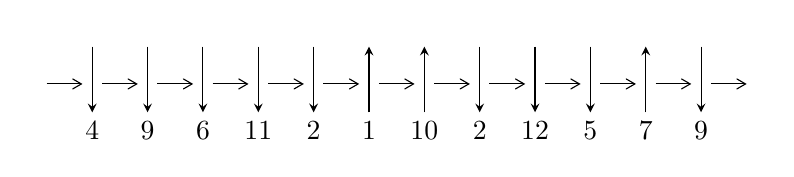
\begin{tikzpicture}[x=20pt, y=17pt]
	% nodes
	\node (C0) at (0, 0) {};
	\node (C1) at (1, 0) {};
	\node (C1U) at (1, +1) {};
	\node (C1D) at (1, -1) {4};

	\node (C2) at (2, 0) {};
	\node (C2U) at (2, +1) {};
	\node (C2D) at (2, -1) {9};

	\node (C3) at (3, 0) {};
	\node (C3U) at (3, +1) {};
	\node (C3D) at (3, -1) {6};

	\node (C4) at (4, 0) {};
	\node (C4U) at (4, +1) {};
	\node (C4D) at (4, -1) {11};

	\node (C5) at (5, 0) {};
	\node (C5U) at (5, +1) {};
	\node (C5D) at (5, -1) {2};

	\node (C6) at (6, 0) {};
	\node (C6U) at (6, +1) {};
	\node (C6D) at (6, -1) {1};

	\node (C7) at (7, 0) {};
	\node (C7U) at (7, +1) {};
	\node (C7D) at (7, -1) {10};

	\node (C8) at (8, 0) {};
	\node (C8U) at (8, +1) {};
	\node (C8D) at (8, -1) {2};

	\node (C9) at (9, 0) {};
	\node (C9U) at (9, +1) {};
	\node (C9D) at (9, -1) {12};

	\node (C10) at (10, 0) {};
	\node (C10U) at (10, +1) {};
	\node (C10D) at (10, -1) {5};

	\node (C11) at (11, 0) {};
	\node (C11U) at (11, +1) {};
	\node (C11D) at (11, -1) {7};

	\node (C12) at (12, 0) {};
	\node (C12U) at (12, +1) {};
	\node (C12D) at (12, -1) {9};
	\node (C13) at (13, 0) {};

	% arrows
	\draw[->,>={angle 60}]
	(C0) edge (C1) (C1) edge (C2) (C2) edge (C3) (C3) edge (C4) (C4) edge (C5) (C5) edge (C6) (C6) edge (C7) (C7) edge (C8) (C8) edge (C9) (C9) edge (C10) (C10) edge (C11) (C11) edge (C12) (C12) edge (C13) ;	\draw[->,>=stealth]
	(C1U) edge (C1D) (C2U) edge (C2D) (C3U) edge (C3D) (C4U) edge (C4D) (C5U) edge (C5D) (C6D) edge (C6U) (C7D) edge (C7U) (C8U) edge (C8D) (C9U) edge (C9D) (C10U) edge (C10D) (C11D) edge (C11U) (C12U) edge (C12D) ;
	\end{tikzpicture} \\
\hhline{~~} \\& 
\textbf{Solving Sequence} \\ \cline{2-2} 
 &
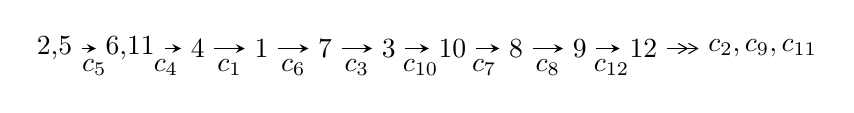
\begin{tikzpicture}[x=23pt, y=7pt]
	% node
	\node (A0) at (-1/8, 0) {2,5};
	\node (A1) at (17/16, 0) {6,11};
	\node (A2) at (17/8, 0) {4};
	\node (A3) at (25/8, 0) {1};
	\node (A4) at (33/8, 0) {7};
	\node (A5) at (41/8, 0) {3};
	\node (A6) at (49/8, 0) {10};
	\node (A7) at (57/8, 0) {8};
	\node (A8) at (65/8, 0) {9};
	\node (A9) at (73/8, 0) {12};
	\node (C1) at (1/2, -1) {$c_{5}$};
	\node (C2) at (13/8, -1) {$c_{4}$};
	\node (C3) at (21/8, -1) {$c_{1}$};
	\node (C4) at (29/8, -1) {$c_{6}$};
	\node (C5) at (37/8, -1) {$c_{3}$};
	\node (C6) at (45/8, -1) {$c_{10}$};
	\node (C7) at (53/8, -1) {$c_{7}$};
	\node (C8) at (61/8, -1) {$c_{8}$};
	\node (C9) at (69/8, -1) {$c_{12}$};
	\node (A10) at (11, 0) {$c_{2},c_{9},c_{11}$};

	% edge
	\draw[->,>=stealth]	
	(A0) edge (A1) (A1) edge (A2) (A2) edge (A3) (A3) edge (A4) (A4) edge (A5) (A5) edge (A6) (A6) edge (A7) (A7) edge (A8) (A8) edge (A9) ;
	\draw[->>,>={angle 60}]	
	(A9) edge (A10);
\end{tikzpicture} \\ 

\end{tabular} \\

\footnotetext{
The image of knot diagram is generated by the software ``\textbf{Draw programme}" developed by Andrew Bartholomew(\url{http://www.layer8.co.uk/maths/draw/index.htm\#Running-draw}), where we modified some parts for our purpose(\url{https://github.com/CATsTAILs/LinksPainter}).
}\phantom \\ \newline 
\centering \textbf{Ideals for irreducible components\footnotemark of $X_{\text{par}}$} 
 
\begin{align*}
I^u_{1}&=\langle 
-6.49376\times10^{915} u^{101}+1.36988\times10^{916} u^{100}+\cdots+1.53445\times10^{923} b+2.64941\times10^{921},\\
\phantom{I^u_{1}}&\phantom{= \langle  }9.51197\times10^{922} u^{101}-1.85089\times10^{923} u^{100}+\cdots+6.71402\times10^{929} a-2.46247\times10^{930},\\
\phantom{I^u_{1}}&\phantom{= \langle  }u^{102}-2 u^{101}+\cdots+8420092 u-4375517\rangle \\
I^u_{2}&=\langle 
-2.56336\times10^{105} u^{42}-7.11346\times10^{105} u^{41}+\cdots+2.75081\times10^{102} b+1.14602\times10^{106},\\
\phantom{I^u_{2}}&\phantom{= \langle  }-1.01986\times10^{106} u^{42}-2.86981\times10^{106} u^{41}+\cdots+2.75081\times10^{102} a+5.56514\times10^{106},\\
\phantom{I^u_{2}}&\phantom{= \langle  }u^{43}+3 u^{42}+\cdots-28 u-1\rangle \\
\\
\end{align*}
\raggedright * 2 irreducible components of $\dim_{\mathbb{C}}=0$, with total 145 representations.\\
\footnotetext{All coefficients of polynomials are rational numbers. But the coefficients are sometimes approximated in decimal forms when there is not enough margin.}
\newpage
\renewcommand{\arraystretch}{1}
\centering \section*{I. $I^u_{1}= \langle -6.49\times10^{915} u^{101}+1.37\times10^{916} u^{100}+\cdots+1.53\times10^{923} b+2.65\times10^{921},\;9.51\times10^{922} u^{101}-1.85\times10^{923} u^{100}+\cdots+6.71\times10^{929} a-2.46\times10^{930},\;u^{102}-2 u^{101}+\cdots+8420092 u-4375517 \rangle$}
\flushleft \textbf{(i) Arc colorings}\\
\begin{tabular}{m{7pt} m{180pt} m{7pt} m{180pt} }
\flushright $a_{2}=$&$\begin{pmatrix}0\\u\end{pmatrix}$ \\
\flushright $a_{5}=$&$\begin{pmatrix}1\\0\end{pmatrix}$ \\
\flushright $a_{6}=$&$\begin{pmatrix}1\\u^2\end{pmatrix}$ \\
\flushright $a_{11}=$&$\begin{pmatrix}-1.41673\times10^{-7} u^{101}+2.75676\times10^{-7} u^{100}+\cdots-0.735672 u+3.66764\\4.23197\times10^{-8} u^{101}-8.92749\times10^{-8} u^{100}+\cdots+0.936625 u-0.0172662\end{pmatrix}$ \\
\flushright $a_{4}=$&$\begin{pmatrix}-2.05443\times10^{-7} u^{101}+4.26875\times10^{-7} u^{100}+\cdots-22.2758 u-0.835178\\1.00487\times10^{-8} u^{101}-2.32210\times10^{-8} u^{100}+\cdots+3.61648 u+0.302504\end{pmatrix}$ \\
\flushright $a_{1}=$&$\begin{pmatrix}1.76309\times10^{-7} u^{101}-3.91156\times10^{-7} u^{100}+\cdots+12.8200 u+0.790115\\7.30728\times10^{-9} u^{101}-1.35715\times10^{-8} u^{100}+\cdots+0.427561 u-0.351917\end{pmatrix}$ \\
\flushright $a_{7}=$&$\begin{pmatrix}1.25051\times10^{-7} u^{101}-2.82188\times10^{-7} u^{100}+\cdots+22.0518 u-1.94211\\-5.85977\times10^{-9} u^{101}+1.76200\times10^{-8} u^{100}+\cdots-0.0550341 u+0.402167\end{pmatrix}$ \\
\flushright $a_{3}=$&$\begin{pmatrix}-1.93843\times10^{-7} u^{101}+4.01235\times10^{-7} u^{100}+\cdots-17.6257 u-0.602635\\8.79886\times10^{-9} u^{101}-2.00013\times10^{-8} u^{100}+\cdots+3.68779 u+0.291821\end{pmatrix}$ \\
\flushright $a_{10}=$&$\begin{pmatrix}-9.93535\times10^{-8} u^{101}+1.86401\times10^{-7} u^{100}+\cdots+0.200954 u+3.65038\\4.23197\times10^{-8} u^{101}-8.92749\times10^{-8} u^{100}+\cdots+0.936625 u-0.0172662\end{pmatrix}$ \\
\flushright $a_{8}=$&$\begin{pmatrix}1.14273\times10^{-9} u^{101}-3.30148\times10^{-8} u^{100}+\cdots+5.30898 u-5.51886\\1.90361\times10^{-10} u^{101}-2.90964\times10^{-9} u^{100}+\cdots+3.74212 u+0.640727\end{pmatrix}$ \\
\flushright $a_{9}=$&$\begin{pmatrix}1.14273\times10^{-9} u^{101}-3.30148\times10^{-8} u^{100}+\cdots+5.30898 u-5.51886\\3.20935\times10^{-9} u^{101}-8.91944\times10^{-9} u^{100}+\cdots+4.00586 u+0.506270\end{pmatrix}$ \\
\flushright $a_{12}=$&$\begin{pmatrix}7.49943\times10^{-8} u^{101}-1.62627\times10^{-7} u^{100}+\cdots+31.5583 u+2.87114\\1.58743\times10^{-8} u^{101}-2.92506\times10^{-8} u^{100}+\cdots-3.56647 u+0.364248\end{pmatrix}$\\&\end{tabular}
\flushleft \textbf{(ii) Obstruction class $= -1$}\\~\\
\flushleft \textbf{(iii) Cusp Shapes $= -7.07644\times10^{-8} u^{101}+9.56061\times10^{-8} u^{100}+\cdots+4.68523 u-4.86639$}\\~\\
\newpage\renewcommand{\arraystretch}{1}
\flushleft \textbf{(iv) u-Polynomials at the component}\newline \\
\begin{tabular}{m{50pt}|m{274pt}}
Crossings & \hspace{64pt}u-Polynomials at each crossing \\
\hline $$\begin{aligned}c_{1}\end{aligned}$$&$\begin{aligned}
&u^{102}-6 u^{101}+\cdots-13 u+1
\end{aligned}$\\
\hline $$\begin{aligned}c_{2},c_{8}\end{aligned}$$&$\begin{aligned}
&u^{102}+3 u^{101}+\cdots-2892097 u-211369
\end{aligned}$\\
\hline $$\begin{aligned}c_{3}\end{aligned}$$&$\begin{aligned}
&u^{102}-12 u^{101}+\cdots+44683235 u-49868279
\end{aligned}$\\
\hline $$\begin{aligned}c_{4},c_{10}\end{aligned}$$&$\begin{aligned}
&u^{102}-2 u^{101}+\cdots-35912 u-22021
\end{aligned}$\\
\hline $$\begin{aligned}c_{5}\end{aligned}$$&$\begin{aligned}
&u^{102}-2 u^{101}+\cdots+8420092 u-4375517
\end{aligned}$\\
\hline $$\begin{aligned}c_{6}\end{aligned}$$&$\begin{aligned}
&u^{102}+4 u^{101}+\cdots-10237986 u-1560347
\end{aligned}$\\
\hline $$\begin{aligned}c_{7}\end{aligned}$$&$\begin{aligned}
&u^{102}+6 u^{101}+\cdots+1478240064 u+120775104
\end{aligned}$\\
\hline $$\begin{aligned}c_{9},c_{12}\end{aligned}$$&$\begin{aligned}
&u^{102}-3 u^{101}+\cdots+17272 u+2887
\end{aligned}$\\
\hline $$\begin{aligned}c_{11}\end{aligned}$$&$\begin{aligned}
&u^{102}-3 u^{101}+\cdots+4237 u+211
\end{aligned}$\\
\hline
\end{tabular}\\~\\
\newpage\renewcommand{\arraystretch}{1}
\flushleft \textbf{(v) Riley Polynomials at the component}\newline \\
\begin{tabular}{m{50pt}|m{274pt}}
Crossings & \hspace{64pt}Riley Polynomials at each crossing \\
\hline $$\begin{aligned}c_{1}\end{aligned}$$&$\begin{aligned}
&y^{102}-26 y^{101}+\cdots+3 y+1
\end{aligned}$\\
\hline $$\begin{aligned}c_{2},c_{8}\end{aligned}$$&$\begin{aligned}
&y^{102}+93 y^{101}+\cdots+186729819967 y+44676854161
\end{aligned}$\\
\hline $$\begin{aligned}c_{3}\end{aligned}$$&$\begin{aligned}
&y^{102}+34 y^{101}+\cdots+32423793145983377 y+2486845250421841
\end{aligned}$\\
\hline $$\begin{aligned}c_{4},c_{10}\end{aligned}$$&$\begin{aligned}
&y^{102}+72 y^{101}+\cdots+13249120960 y+484924441
\end{aligned}$\\
\hline $$\begin{aligned}c_{5}\end{aligned}$$&$\begin{aligned}
&y^{102}+34 y^{101}+\cdots-851807783365426 y+19145149017289
\end{aligned}$\\
\hline $$\begin{aligned}c_{6}\end{aligned}$$&$\begin{aligned}
&y^{102}-42 y^{101}+\cdots-69780057418512 y+2434682760409
\end{aligned}$\\
\hline $$\begin{aligned}c_{7}\end{aligned}$$&$\begin{aligned}
&y^{102}-56 y^{101}+\cdots-839500422669637632 y+14586625746210816
\end{aligned}$\\
\hline $$\begin{aligned}c_{9},c_{12}\end{aligned}$$&$\begin{aligned}
&y^{102}+83 y^{101}+\cdots-227405716 y+8334769
\end{aligned}$\\
\hline $$\begin{aligned}c_{11}\end{aligned}$$&$\begin{aligned}
&y^{102}+13 y^{101}+\cdots-9748489 y+44521
\end{aligned}$\\
\hline
\end{tabular}\\~\\
\newpage\flushleft \textbf{(vi) Complex Volumes and Cusp Shapes}
$$\begin{array}{c|c|c}  
\text{Solutions to }I^u_{1}& \I (\text{vol} + \sqrt{-1}CS) & \text{Cusp shape}\\
 \hline 
\begin{aligned}
u &= \phantom{-}0.578447 + 0.812318 I \\
a &= \phantom{-}0.270355 + 0.352500 I \\
b &= \phantom{-}0.654512 + 0.190971 I\end{aligned}
 & \phantom{-}2.61090 - 2.24156 I & \phantom{-0.000000 } 0 \\ \hline\begin{aligned}
u &= \phantom{-}0.578447 - 0.812318 I \\
a &= \phantom{-}0.270355 - 0.352500 I \\
b &= \phantom{-}0.654512 - 0.190971 I\end{aligned}
 & \phantom{-}2.61090 + 2.24156 I & \phantom{-0.000000 } 0 \\ \hline\begin{aligned}
u &= -0.640649 + 0.738622 I \\
a &= -1.40013 - 0.36420 I \\
b &= \phantom{-}0.178260 + 1.219860 I\end{aligned}
 & -1.36519 - 4.12170 I & \phantom{-0.000000 } 0 \\ \hline\begin{aligned}
u &= -0.640649 - 0.738622 I \\
a &= -1.40013 + 0.36420 I \\
b &= \phantom{-}0.178260 - 1.219860 I\end{aligned}
 & -1.36519 + 4.12170 I & \phantom{-0.000000 } 0 \\ \hline\begin{aligned}
u &= \phantom{-}0.785103 + 0.573070 I \\
a &= \phantom{-}1.26596 - 2.01109 I \\
b &= \phantom{-}0.477218 + 1.053040 I\end{aligned}
 & -1.44120 - 6.31655 I & \phantom{-0.000000 } 0 \\ \hline\begin{aligned}
u &= \phantom{-}0.785103 - 0.573070 I \\
a &= \phantom{-}1.26596 + 2.01109 I \\
b &= \phantom{-}0.477218 - 1.053040 I\end{aligned}
 & -1.44120 + 6.31655 I & \phantom{-0.000000 } 0 \\ \hline\begin{aligned}
u &= \phantom{-}0.388226 + 0.961377 I \\
a &= -0.492122 - 0.348872 I \\
b &= -1.052880 - 0.601333 I\end{aligned}
 & \phantom{-}5.87214 - 3.57059 I & \phantom{-0.000000 } 0 \\ \hline\begin{aligned}
u &= \phantom{-}0.388226 - 0.961377 I \\
a &= -0.492122 + 0.348872 I \\
b &= -1.052880 + 0.601333 I\end{aligned}
 & \phantom{-}5.87214 + 3.57059 I & \phantom{-0.000000 } 0 \\ \hline\begin{aligned}
u &= -0.893646 + 0.337908 I \\
a &= -0.204247 + 0.597815 I \\
b &= \phantom{-}0.607279 + 0.413909 I\end{aligned}
 & -3.27710 + 2.11779 I & -16.4652 + 0. I\phantom{ +0.000000I} \\ \hline\begin{aligned}
u &= -0.893646 - 0.337908 I \\
a &= -0.204247 - 0.597815 I \\
b &= \phantom{-}0.607279 - 0.413909 I\end{aligned}
 & -3.27710 - 2.11779 I & -16.4652 + 0. I\phantom{ +0.000000I}\\
 \hline 
 \end{array}$$\newpage$$\begin{array}{c|c|c}  
\text{Solutions to }I^u_{1}& \I (\text{vol} + \sqrt{-1}CS) & \text{Cusp shape}\\
 \hline 
\begin{aligned}
u &= \phantom{-}0.830323 + 0.440927 I \\
a &= \phantom{-}0.159520 + 0.434049 I \\
b &= \phantom{-}0.197571 + 0.786043 I\end{aligned}
 & \phantom{-}2.90646 - 1.74561 I & \phantom{-0.000000 } 0 \\ \hline\begin{aligned}
u &= \phantom{-}0.830323 - 0.440927 I \\
a &= \phantom{-}0.159520 - 0.434049 I \\
b &= \phantom{-}0.197571 - 0.786043 I\end{aligned}
 & \phantom{-}2.90646 + 1.74561 I & \phantom{-0.000000 } 0 \\ \hline\begin{aligned}
u &= \phantom{-}0.536482 + 0.767816 I \\
a &= \phantom{-}0.198515 - 1.013870 I \\
b &= -0.575438 + 0.925227 I\end{aligned}
 & -0.66291 + 3.42491 I & -6.00000 + 0. I\phantom{ +0.000000I} \\ \hline\begin{aligned}
u &= \phantom{-}0.536482 - 0.767816 I \\
a &= \phantom{-}0.198515 + 1.013870 I \\
b &= -0.575438 - 0.925227 I\end{aligned}
 & -0.66291 - 3.42491 I & -6.00000 + 0. I\phantom{ +0.000000I} \\ \hline\begin{aligned}
u &= -0.927521 + 0.012182 I \\
a &= -0.116711 - 0.927791 I \\
b &= -0.29093 + 1.44713 I\end{aligned}
 & -1.66180 + 0.53067 I & -14.1328 + 9.6811 I \\ \hline\begin{aligned}
u &= -0.927521 - 0.012182 I \\
a &= -0.116711 + 0.927791 I \\
b &= -0.29093 - 1.44713 I\end{aligned}
 & -1.66180 - 0.53067 I & -14.1328 - 9.6811 I \\ \hline\begin{aligned}
u &= \phantom{-}0.462524 + 0.975614 I \\
a &= -0.095337 + 1.036880 I \\
b &= \phantom{-}0.607615 - 1.043800 I\end{aligned}
 & \phantom{-}1.67405 + 8.43926 I & \phantom{-0.000000 } 0 \\ \hline\begin{aligned}
u &= \phantom{-}0.462524 - 0.975614 I \\
a &= -0.095337 - 1.036880 I \\
b &= \phantom{-}0.607615 + 1.043800 I\end{aligned}
 & \phantom{-}1.67405 - 8.43926 I & \phantom{-0.000000 } 0 \\ \hline\begin{aligned}
u &= -0.891060 + 0.018793 I \\
a &= -0.394094 + 0.410206 I \\
b &= -0.975211 + 0.681945 I\end{aligned}
 & \phantom{-}0.997093 + 0.093900 I & -3.60215 + 1.98192 I \\ \hline\begin{aligned}
u &= -0.891060 - 0.018793 I \\
a &= -0.394094 - 0.410206 I \\
b &= -0.975211 - 0.681945 I\end{aligned}
 & \phantom{-}0.997093 - 0.093900 I & -3.60215 - 1.98192 I\\
 \hline 
 \end{array}$$\newpage$$\begin{array}{c|c|c}  
\text{Solutions to }I^u_{1}& \I (\text{vol} + \sqrt{-1}CS) & \text{Cusp shape}\\
 \hline 
\begin{aligned}
u &= \phantom{-}0.640255 + 0.960663 I \\
a &= -0.35799 + 1.48956 I \\
b &= -0.185489 - 1.251300 I\end{aligned}
 & \phantom{-}3.04751 - 2.50600 I & \phantom{-0.000000 } 0 \\ \hline\begin{aligned}
u &= \phantom{-}0.640255 - 0.960663 I \\
a &= -0.35799 - 1.48956 I \\
b &= -0.185489 + 1.251300 I\end{aligned}
 & \phantom{-}3.04751 + 2.50600 I & \phantom{-0.000000 } 0 \\ \hline\begin{aligned}
u &= \phantom{-}1.083950 + 0.498268 I \\
a &= \phantom{-}0.467119 - 0.389987 I \\
b &= \phantom{-}0.171905 - 0.609109 I\end{aligned}
 & \phantom{-}4.20152 - 5.01214 I & \phantom{-0.000000 } 0 \\ \hline\begin{aligned}
u &= \phantom{-}1.083950 - 0.498268 I \\
a &= \phantom{-}0.467119 + 0.389987 I \\
b &= \phantom{-}0.171905 + 0.609109 I\end{aligned}
 & \phantom{-}4.20152 + 5.01214 I & \phantom{-0.000000 } 0 \\ \hline\begin{aligned}
u &= \phantom{-}1.22973\phantom{ +0.000000I} \\
a &= \phantom{-}1.85972\phantom{ +0.000000I} \\
b &= \phantom{-}1.57058\phantom{ +0.000000I}\end{aligned}
 & -7.95878\phantom{ +0.000000I} & \phantom{-0.000000 } 0 \\ \hline\begin{aligned}
u &= \phantom{-}0.758319 + 0.976081 I \\
a &= \phantom{-}0.443026 - 0.834537 I \\
b &= \phantom{-}0.61949 + 1.38371 I\end{aligned}
 & \phantom{-}4.95097 - 3.85407 I & \phantom{-0.000000 } 0 \\ \hline\begin{aligned}
u &= \phantom{-}0.758319 - 0.976081 I \\
a &= \phantom{-}0.443026 + 0.834537 I \\
b &= \phantom{-}0.61949 - 1.38371 I\end{aligned}
 & \phantom{-}4.95097 + 3.85407 I & \phantom{-0.000000 } 0 \\ \hline\begin{aligned}
u &= \phantom{-}0.931306 + 0.828752 I \\
a &= \phantom{-}0.70992 - 1.24219 I \\
b &= \phantom{-}0.306421 + 1.241220 I\end{aligned}
 & \phantom{-}5.33219 - 6.63790 I & \phantom{-0.000000 } 0 \\ \hline\begin{aligned}
u &= \phantom{-}0.931306 - 0.828752 I \\
a &= \phantom{-}0.70992 + 1.24219 I \\
b &= \phantom{-}0.306421 - 1.241220 I\end{aligned}
 & \phantom{-}5.33219 + 6.63790 I & \phantom{-0.000000 } 0 \\ \hline\begin{aligned}
u &= \phantom{-}0.021438 + 1.263280 I \\
a &= \phantom{-}0.77335 - 1.52919 I \\
b &= -0.037608 + 1.187630 I\end{aligned}
 & \phantom{-}4.98554 + 1.41809 I & \phantom{-0.000000 } 0\\
 \hline 
 \end{array}$$\newpage$$\begin{array}{c|c|c}  
\text{Solutions to }I^u_{1}& \I (\text{vol} + \sqrt{-1}CS) & \text{Cusp shape}\\
 \hline 
\begin{aligned}
u &= \phantom{-}0.021438 - 1.263280 I \\
a &= \phantom{-}0.77335 + 1.52919 I \\
b &= -0.037608 - 1.187630 I\end{aligned}
 & \phantom{-}4.98554 - 1.41809 I & \phantom{-0.000000 } 0 \\ \hline\begin{aligned}
u &= -0.604900 + 0.398404 I \\
a &= \phantom{-}1.50133 + 0.47327 I \\
b &= -0.314470 + 0.216566 I\end{aligned}
 & \phantom{-}1.35379 + 5.01097 I & -4.29413 - 5.82522 I \\ \hline\begin{aligned}
u &= -0.604900 - 0.398404 I \\
a &= \phantom{-}1.50133 - 0.47327 I \\
b &= -0.314470 - 0.216566 I\end{aligned}
 & \phantom{-}1.35379 - 5.01097 I & -4.29413 + 5.82522 I \\ \hline\begin{aligned}
u &= -1.081470 + 0.701710 I \\
a &= -0.727456 - 0.787717 I \\
b &= \phantom{-}0.215463 + 0.924006 I\end{aligned}
 & -0.61960 - 3.63133 I & \phantom{-0.000000 } 0 \\ \hline\begin{aligned}
u &= -1.081470 - 0.701710 I \\
a &= -0.727456 + 0.787717 I \\
b &= \phantom{-}0.215463 - 0.924006 I\end{aligned}
 & -0.61960 + 3.63133 I & \phantom{-0.000000 } 0 \\ \hline\begin{aligned}
u &= -1.119540 + 0.708835 I \\
a &= -0.124837 - 0.074168 I \\
b &= -0.744192 - 0.630943 I\end{aligned}
 & \phantom{-}1.11900 + 1.01088 I & \phantom{-0.000000 } 0 \\ \hline\begin{aligned}
u &= -1.119540 - 0.708835 I \\
a &= -0.124837 + 0.074168 I \\
b &= -0.744192 + 0.630943 I\end{aligned}
 & \phantom{-}1.11900 - 1.01088 I & \phantom{-0.000000 } 0 \\ \hline\begin{aligned}
u &= -0.621598 + 1.198780 I \\
a &= \phantom{-}0.16801 + 1.81726 I \\
b &= \phantom{-}0.207158 - 1.166130 I\end{aligned}
 & \phantom{-}6.23243 + 6.77828 I & \phantom{-0.000000 } 0 \\ \hline\begin{aligned}
u &= -0.621598 - 1.198780 I \\
a &= \phantom{-}0.16801 - 1.81726 I \\
b &= \phantom{-}0.207158 + 1.166130 I\end{aligned}
 & \phantom{-}6.23243 - 6.77828 I & \phantom{-0.000000 } 0 \\ \hline\begin{aligned}
u &= \phantom{-}0.622914 + 1.201910 I \\
a &= -0.820504 + 0.851583 I \\
b &= -0.38872 - 1.58447 I\end{aligned}
 & \phantom{-}8.17405 - 2.71521 I & \phantom{-0.000000 } 0\\
 \hline 
 \end{array}$$\newpage$$\begin{array}{c|c|c}  
\text{Solutions to }I^u_{1}& \I (\text{vol} + \sqrt{-1}CS) & \text{Cusp shape}\\
 \hline 
\begin{aligned}
u &= \phantom{-}0.622914 - 1.201910 I \\
a &= -0.820504 - 0.851583 I \\
b &= -0.38872 + 1.58447 I\end{aligned}
 & \phantom{-}8.17405 + 2.71521 I & \phantom{-0.000000 } 0 \\ \hline\begin{aligned}
u &= -0.117787 + 0.635374 I \\
a &= -0.234595 - 1.221780 I \\
b &= -0.556422 + 0.759811 I\end{aligned}
 & -1.28229 + 1.29324 I & -7.96430 - 5.38509 I \\ \hline\begin{aligned}
u &= -0.117787 - 0.635374 I \\
a &= -0.234595 + 1.221780 I \\
b &= -0.556422 - 0.759811 I\end{aligned}
 & -1.28229 - 1.29324 I & -7.96430 + 5.38509 I \\ \hline\begin{aligned}
u &= -0.637979 + 0.054784 I \\
a &= \phantom{-}0.94673 - 2.63004 I \\
b &= \phantom{-}0.196852 - 0.700152 I\end{aligned}
 & -3.63718 - 2.68680 I & -19.7191 + 1.0309 I \\ \hline\begin{aligned}
u &= -0.637979 - 0.054784 I \\
a &= \phantom{-}0.94673 + 2.63004 I \\
b &= \phantom{-}0.196852 + 0.700152 I\end{aligned}
 & -3.63718 + 2.68680 I & -19.7191 - 1.0309 I \\ \hline\begin{aligned}
u &= -0.630129\phantom{ +0.000000I} \\
a &= -0.281979\phantom{ +0.000000I} \\
b &= -0.482624\phantom{ +0.000000I}\end{aligned}
 & -0.874381\phantom{ +0.000000I} & -11.7060\phantom{ +0.000000I} \\ \hline\begin{aligned}
u &= \phantom{-}0.381446 + 1.333600 I \\
a &= \phantom{-}0.577005 - 0.792791 I \\
b &= \phantom{-}0.48223 + 1.69159 I\end{aligned}
 & \phantom{-}13.5875 + 4.2210 I & \phantom{-0.000000 } 0 \\ \hline\begin{aligned}
u &= \phantom{-}0.381446 - 1.333600 I \\
a &= \phantom{-}0.577005 + 0.792791 I \\
b &= \phantom{-}0.48223 - 1.69159 I\end{aligned}
 & \phantom{-}13.5875 - 4.2210 I & \phantom{-0.000000 } 0 \\ \hline\begin{aligned}
u &= \phantom{-}1.280040 + 0.559635 I \\
a &= -1.26835 + 1.09747 I \\
b &= -0.676662 - 0.970337 I\end{aligned}
 & \phantom{-}2.02370 - 6.46913 I & \phantom{-0.000000 } 0 \\ \hline\begin{aligned}
u &= \phantom{-}1.280040 - 0.559635 I \\
a &= -1.26835 - 1.09747 I \\
b &= -0.676662 + 0.970337 I\end{aligned}
 & \phantom{-}2.02370 + 6.46913 I & \phantom{-0.000000 } 0\\
 \hline 
 \end{array}$$\newpage$$\begin{array}{c|c|c}  
\text{Solutions to }I^u_{1}& \I (\text{vol} + \sqrt{-1}CS) & \text{Cusp shape}\\
 \hline 
\begin{aligned}
u &= \phantom{-}0.114976 + 1.398030 I \\
a &= -0.070057 - 0.419974 I \\
b &= -1.45170 + 0.09247 I\end{aligned}
 & \phantom{-}1.96391 - 4.09956 I & \phantom{-0.000000 } 0 \\ \hline\begin{aligned}
u &= \phantom{-}0.114976 - 1.398030 I \\
a &= -0.070057 + 0.419974 I \\
b &= -1.45170 - 0.09247 I\end{aligned}
 & \phantom{-}1.96391 + 4.09956 I & \phantom{-0.000000 } 0 \\ \hline\begin{aligned}
u &= \phantom{-}0.85618 + 1.13679 I \\
a &= \phantom{-}0.994333 - 0.607763 I \\
b &= \phantom{-}0.45510 + 1.40983 I\end{aligned}
 & \phantom{-}12.8090 - 9.7238 I & \phantom{-0.000000 } 0 \\ \hline\begin{aligned}
u &= \phantom{-}0.85618 - 1.13679 I \\
a &= \phantom{-}0.994333 + 0.607763 I \\
b &= \phantom{-}0.45510 - 1.40983 I\end{aligned}
 & \phantom{-}12.8090 + 9.7238 I & \phantom{-0.000000 } 0 \\ \hline\begin{aligned}
u &= \phantom{-}0.434355 + 0.370831 I \\
a &= -0.81976 - 1.90229 I \\
b &= \phantom{-}0.143362 + 0.620182 I\end{aligned}
 & -0.86396 + 1.69582 I & -4.56303 - 2.55235 I \\ \hline\begin{aligned}
u &= \phantom{-}0.434355 - 0.370831 I \\
a &= -0.81976 + 1.90229 I \\
b &= \phantom{-}0.143362 - 0.620182 I\end{aligned}
 & -0.86396 - 1.69582 I & -4.56303 + 2.55235 I \\ \hline\begin{aligned}
u &= \phantom{-}1.28469 + 0.69073 I \\
a &= -0.315215 + 0.773825 I \\
b &= -0.55875 - 1.68138 I\end{aligned}
 & \phantom{-}9.05761 - 6.51883 I & \phantom{-0.000000 } 0 \\ \hline\begin{aligned}
u &= \phantom{-}1.28469 - 0.69073 I \\
a &= -0.315215 - 0.773825 I \\
b &= -0.55875 + 1.68138 I\end{aligned}
 & \phantom{-}9.05761 + 6.51883 I & \phantom{-0.000000 } 0 \\ \hline\begin{aligned}
u &= \phantom{-}0.33639 + 1.43648 I \\
a &= -0.213568 - 1.280870 I \\
b &= -0.040602 + 1.409330 I\end{aligned}
 & \phantom{-}8.11805 + 0.97622 I & \phantom{-0.000000 } 0 \\ \hline\begin{aligned}
u &= \phantom{-}0.33639 - 1.43648 I \\
a &= -0.213568 + 1.280870 I \\
b &= -0.040602 - 1.409330 I\end{aligned}
 & \phantom{-}8.11805 - 0.97622 I & \phantom{-0.000000 } 0\\
 \hline 
 \end{array}$$\newpage$$\begin{array}{c|c|c}  
\text{Solutions to }I^u_{1}& \I (\text{vol} + \sqrt{-1}CS) & \text{Cusp shape}\\
 \hline 
\begin{aligned}
u &= -0.467785 + 0.056572 I \\
a &= \phantom{-}0.552988 + 0.784397 I \\
b &= \phantom{-}1.031520 - 0.176518 I\end{aligned}
 & \phantom{-}0.46845 + 3.00397 I & -6.44837 - 8.33144 I \\ \hline\begin{aligned}
u &= -0.467785 - 0.056572 I \\
a &= \phantom{-}0.552988 - 0.784397 I \\
b &= \phantom{-}1.031520 + 0.176518 I\end{aligned}
 & \phantom{-}0.46845 - 3.00397 I & -6.44837 + 8.33144 I \\ \hline\begin{aligned}
u &= \phantom{-}0.62649 + 1.43614 I \\
a &= \phantom{-}0.131084 + 0.242971 I \\
b &= \phantom{-}1.340060 - 0.085585 I\end{aligned}
 & \phantom{-}7.81773 - 11.25560 I & \phantom{-0.000000 } 0 \\ \hline\begin{aligned}
u &= \phantom{-}0.62649 - 1.43614 I \\
a &= \phantom{-}0.131084 - 0.242971 I \\
b &= \phantom{-}1.340060 + 0.085585 I\end{aligned}
 & \phantom{-}7.81773 + 11.25560 I & \phantom{-0.000000 } 0 \\ \hline\begin{aligned}
u &= \phantom{-}0.206203 + 0.378033 I \\
a &= -1.04319 + 1.92882 I \\
b &= \phantom{-}0.444813 - 0.992717 I\end{aligned}
 & \phantom{-}3.48779 + 1.18350 I & \phantom{-}0.466384 - 0.755659 I \\ \hline\begin{aligned}
u &= \phantom{-}0.206203 - 0.378033 I \\
a &= -1.04319 - 1.92882 I \\
b &= \phantom{-}0.444813 + 0.992717 I\end{aligned}
 & \phantom{-}3.48779 - 1.18350 I & \phantom{-}0.466384 + 0.755659 I \\ \hline\begin{aligned}
u &= -1.56760 + 0.22766 I \\
a &= \phantom{-}0.047477 + 0.185643 I \\
b &= -0.042340 - 1.045710 I\end{aligned}
 & -0.10095 + 2.17396 I & \phantom{-0.000000 } 0 \\ \hline\begin{aligned}
u &= -1.56760 - 0.22766 I \\
a &= \phantom{-}0.047477 - 0.185643 I \\
b &= -0.042340 + 1.045710 I\end{aligned}
 & -0.10095 - 2.17396 I & \phantom{-0.000000 } 0 \\ \hline\begin{aligned}
u &= -0.017667 + 0.390853 I \\
a &= \phantom{-}0.323909 + 1.038640 I \\
b &= \phantom{-}0.939261 - 0.458593 I\end{aligned}
 & -0.03263 - 2.94373 I & \phantom{-}3.57558 + 3.19837 I \\ \hline\begin{aligned}
u &= -0.017667 - 0.390853 I \\
a &= \phantom{-}0.323909 - 1.038640 I \\
b &= \phantom{-}0.939261 + 0.458593 I\end{aligned}
 & -0.03263 + 2.94373 I & \phantom{-}3.57558 - 3.19837 I\\
 \hline 
 \end{array}$$\newpage$$\begin{array}{c|c|c}  
\text{Solutions to }I^u_{1}& \I (\text{vol} + \sqrt{-1}CS) & \text{Cusp shape}\\
 \hline 
\begin{aligned}
u &= \phantom{-}0.60708 + 1.52672 I \\
a &= -0.507253 - 0.219819 I \\
b &= -0.765030 + 0.142961 I\end{aligned}
 & \phantom{-}7.72482 - 1.06832 I & \phantom{-0.000000 } 0 \\ \hline\begin{aligned}
u &= \phantom{-}0.60708 - 1.52672 I \\
a &= -0.507253 + 0.219819 I \\
b &= -0.765030 - 0.142961 I\end{aligned}
 & \phantom{-}7.72482 + 1.06832 I & \phantom{-0.000000 } 0 \\ \hline\begin{aligned}
u &= -0.02581 + 1.67606 I \\
a &= \phantom{-}0.317248 + 0.644991 I \\
b &= \phantom{-}1.065830 - 0.281927 I\end{aligned}
 & \phantom{-}7.60998 + 4.47661 I & \phantom{-0.000000 } 0 \\ \hline\begin{aligned}
u &= -0.02581 - 1.67606 I \\
a &= \phantom{-}0.317248 - 0.644991 I \\
b &= \phantom{-}1.065830 + 0.281927 I\end{aligned}
 & \phantom{-}7.60998 - 4.47661 I & \phantom{-0.000000 } 0 \\ \hline\begin{aligned}
u &= -0.198769 + 0.106085 I \\
a &= \phantom{-}5.94644 + 2.42648 I \\
b &= -0.442931 - 0.691015 I\end{aligned}
 & \phantom{-}1.29275 - 5.13529 I & -4.85647 + 5.39780 I \\ \hline\begin{aligned}
u &= -0.198769 - 0.106085 I \\
a &= \phantom{-}5.94644 - 2.42648 I \\
b &= -0.442931 + 0.691015 I\end{aligned}
 & \phantom{-}1.29275 + 5.13529 I & -4.85647 - 5.39780 I \\ \hline\begin{aligned}
u &= \phantom{-}0.119450 + 0.086603 I \\
a &= \phantom{-}2.80930 + 5.11498 I \\
b &= \phantom{-}0.308645 - 0.973601 I\end{aligned}
 & -0.57388 - 1.45394 I & -5.08577 + 3.51030 I \\ \hline\begin{aligned}
u &= \phantom{-}0.119450 - 0.086603 I \\
a &= \phantom{-}2.80930 - 5.11498 I \\
b &= \phantom{-}0.308645 + 0.973601 I\end{aligned}
 & -0.57388 + 1.45394 I & -5.08577 - 3.51030 I \\ \hline\begin{aligned}
u &= -0.94704 + 1.61116 I \\
a &= \phantom{-}0.324213 + 1.195960 I \\
b &= \phantom{-}0.391276 - 1.259480 I\end{aligned}
 & \phantom{-}6.80887 + 6.18363 I & \phantom{-0.000000 } 0 \\ \hline\begin{aligned}
u &= -0.94704 - 1.61116 I \\
a &= \phantom{-}0.324213 - 1.195960 I \\
b &= \phantom{-}0.391276 + 1.259480 I\end{aligned}
 & \phantom{-}6.80887 - 6.18363 I & \phantom{-0.000000 } 0\\
 \hline 
 \end{array}$$\newpage$$\begin{array}{c|c|c}  
\text{Solutions to }I^u_{1}& \I (\text{vol} + \sqrt{-1}CS) & \text{Cusp shape}\\
 \hline 
\begin{aligned}
u &= \phantom{-}0.14001 + 1.89916 I \\
a &= \phantom{-}0.191102 + 1.151240 I \\
b &= -0.306706 - 1.357360 I\end{aligned}
 & \phantom{-}6.26027 - 8.13426 I & \phantom{-0.000000 } 0 \\ \hline\begin{aligned}
u &= \phantom{-}0.14001 - 1.89916 I \\
a &= \phantom{-}0.191102 - 1.151240 I \\
b &= -0.306706 + 1.357360 I\end{aligned}
 & \phantom{-}6.26027 + 8.13426 I & \phantom{-0.000000 } 0 \\ \hline\begin{aligned}
u &= \phantom{-}0.88769 + 1.73485 I \\
a &= -0.591684 + 0.787057 I \\
b &= -0.195447 - 1.283190 I\end{aligned}
 & \phantom{-}12.14500 - 2.16932 I & \phantom{-0.000000 } 0 \\ \hline\begin{aligned}
u &= \phantom{-}0.88769 - 1.73485 I \\
a &= -0.591684 - 0.787057 I \\
b &= -0.195447 + 1.283190 I\end{aligned}
 & \phantom{-}12.14500 + 2.16932 I & \phantom{-0.000000 } 0 \\ \hline\begin{aligned}
u &= -0.73926 + 1.87167 I \\
a &= -0.186300 - 1.081720 I \\
b &= -0.61651 + 1.47320 I\end{aligned}
 & \phantom{-}6.57040 + 11.23110 I & \phantom{-0.000000 } 0 \\ \hline\begin{aligned}
u &= -0.73926 - 1.87167 I \\
a &= -0.186300 + 1.081720 I \\
b &= -0.61651 - 1.47320 I\end{aligned}
 & \phantom{-}6.57040 - 11.23110 I & \phantom{-0.000000 } 0 \\ \hline\begin{aligned}
u &= \phantom{-}1.94506 + 0.57389 I \\
a &= \phantom{-}0.018583 - 0.755361 I \\
b &= -0.204489 + 0.773130 I\end{aligned}
 & -3.78120 + 1.28591 I & \phantom{-0.000000 } 0 \\ \hline\begin{aligned}
u &= \phantom{-}1.94506 - 0.57389 I \\
a &= \phantom{-}0.018583 + 0.755361 I \\
b &= -0.204489 - 0.773130 I\end{aligned}
 & -3.78120 - 1.28591 I & \phantom{-0.000000 } 0 \\ \hline\begin{aligned}
u &= -1.16309 + 1.83888 I \\
a &= -0.168805 - 1.016590 I \\
b &= -0.37611 + 1.48026 I\end{aligned}
 & \phantom{-}12.3609 + 8.4412 I & \phantom{-0.000000 } 0 \\ \hline\begin{aligned}
u &= -1.16309 - 1.83888 I \\
a &= -0.168805 + 1.016590 I \\
b &= -0.37611 - 1.48026 I\end{aligned}
 & \phantom{-}12.3609 - 8.4412 I & \phantom{-0.000000 } 0\\
 \hline 
 \end{array}$$\newpage$$\begin{array}{c|c|c}  
\text{Solutions to }I^u_{1}& \I (\text{vol} + \sqrt{-1}CS) & \text{Cusp shape}\\
 \hline 
\begin{aligned}
u &= -1.22621 + 1.83672 I \\
a &= \phantom{-}0.340072 + 1.032140 I \\
b &= \phantom{-}0.64018 - 1.42705 I\end{aligned}
 & \phantom{-}12.0876 + 18.1403 I & \phantom{-0.000000 } 0 \\ \hline\begin{aligned}
u &= -1.22621 - 1.83672 I \\
a &= \phantom{-}0.340072 - 1.032140 I \\
b &= \phantom{-}0.64018 + 1.42705 I\end{aligned}
 & \phantom{-}12.0876 - 18.1403 I & \phantom{-0.000000 } 0 \\ \hline\begin{aligned}
u &= -0.09203 + 2.24603 I \\
a &= \phantom{-}0.030866 + 0.903213 I \\
b &= \phantom{-}0.75635 - 1.46658 I\end{aligned}
 & \phantom{-}10.80000 + 2.52658 I & \phantom{-0.000000 } 0 \\ \hline\begin{aligned}
u &= -0.09203 - 2.24603 I \\
a &= \phantom{-}0.030866 - 0.903213 I \\
b &= \phantom{-}0.75635 + 1.46658 I\end{aligned}
 & \phantom{-}10.80000 - 2.52658 I & \phantom{-0.000000 } 0 \\ \hline\begin{aligned}
u &= \phantom{-}0.26203 + 2.26872 I \\
a &= -0.481013 + 0.837915 I \\
b &= -0.549181 - 1.043110 I\end{aligned}
 & \phantom{-}10.87960 - 2.17273 I & \phantom{-0.000000 } 0 \\ \hline\begin{aligned}
u &= \phantom{-}0.26203 - 2.26872 I \\
a &= -0.481013 - 0.837915 I \\
b &= -0.549181 + 1.043110 I\end{aligned}
 & \phantom{-}10.87960 + 2.17273 I & \phantom{-0.000000 } 0 \\ \hline\begin{aligned}
u &= \phantom{-}2.24269 + 1.11459 I \\
a &= \phantom{-}0.06831 + 1.51402 I \\
b &= -0.026281 - 0.656218 I\end{aligned}
 & \phantom{-}5.73946 + 4.09658 I & \phantom{-0.000000 } 0 \\ \hline\begin{aligned}
u &= \phantom{-}2.24269 - 1.11459 I \\
a &= \phantom{-}0.06831 - 1.51402 I \\
b &= -0.026281 + 0.656218 I\end{aligned}
 & \phantom{-}5.73946 - 4.09658 I & \phantom{-0.000000 } 0 \\ \hline\begin{aligned}
u &= -1.40790 + 2.19475 I \\
a &= -0.447499 - 0.965940 I \\
b &= -0.472802 + 1.188240 I\end{aligned}
 & \phantom{-}10.84730 + 5.64112 I & \phantom{-0.000000 } 0 \\ \hline\begin{aligned}
u &= -1.40790 - 2.19475 I \\
a &= -0.447499 + 0.965940 I \\
b &= -0.472802 - 1.188240 I\end{aligned}
 & \phantom{-}10.84730 - 5.64112 I & \phantom{-0.000000 } 0\\
 \hline 
 \end{array}$$\newpage$$\begin{array}{c|c|c}  
\text{Solutions to }I^u_{1}& \I (\text{vol} + \sqrt{-1}CS) & \text{Cusp shape}\\
 \hline 
\begin{aligned}
u &= -3.27458 + 0.21401 I \\
a &= -0.037805 + 0.627899 I \\
b &= -0.135440 - 1.188390 I\end{aligned}
 & \phantom{-}7.88225 - 5.01987 I & \phantom{-0.000000 } 0 \\ \hline\begin{aligned}
u &= -3.27458 - 0.21401 I \\
a &= -0.037805 - 0.627899 I \\
b &= -0.135440 + 1.188390 I\end{aligned}
 & \phantom{-}7.88225 + 5.01987 I & \phantom{-0.000000 } 0\\
 \hline 
 \end{array}$$\newpage\newpage\renewcommand{\arraystretch}{1}
\centering \section*{II. $I^u_{2}= \langle -2.56\times10^{105} u^{42}-7.11\times10^{105} u^{41}+\cdots+2.75\times10^{102} b+1.15\times10^{106},\;-1.02\times10^{106} u^{42}-2.87\times10^{106} u^{41}+\cdots+2.75\times10^{102} a+5.57\times10^{106},\;u^{43}+3 u^{42}+\cdots-28 u-1 \rangle$}
\flushleft \textbf{(i) Arc colorings}\\
\begin{tabular}{m{7pt} m{180pt} m{7pt} m{180pt} }
\flushright $a_{2}=$&$\begin{pmatrix}0\\u\end{pmatrix}$ \\
\flushright $a_{5}=$&$\begin{pmatrix}1\\0\end{pmatrix}$ \\
\flushright $a_{6}=$&$\begin{pmatrix}1\\u^2\end{pmatrix}$ \\
\flushright $a_{11}=$&$\begin{pmatrix}3707.49 u^{42}+10432.6 u^{41}+\cdots-454966. u-20230.9\\931.857 u^{42}+2585.95 u^{41}+\cdots-97746.0 u-4166.13\end{pmatrix}$ \\
\flushright $a_{4}=$&$\begin{pmatrix}59.1829 u^{42}+145.069 u^{41}+\cdots+5329.50 u+455.518\\702.224 u^{42}+1949.37 u^{41}+\cdots-72606.5 u-3054.31\end{pmatrix}$ \\
\flushright $a_{1}=$&$\begin{pmatrix}1296.36 u^{42}+3722.50 u^{41}+\cdots-196370. u-9266.12\\-242.457 u^{42}-668.784 u^{41}+\cdots+22997.2 u+930.911\end{pmatrix}$ \\
\flushright $a_{7}=$&$\begin{pmatrix}2530.36 u^{42}+7212.55 u^{41}+\cdots-352926. u-16218.1\\261.611 u^{42}+733.273 u^{41}+\cdots-30874.6 u-1366.31\end{pmatrix}$ \\
\flushright $a_{3}=$&$\begin{pmatrix}752.283 u^{42}+2069.21 u^{41}+\cdots-66426.7 u-2566.31\\736.124 u^{42}+2043.82 u^{41}+\cdots-76257.7 u-3209.46\end{pmatrix}$ \\
\flushright $a_{10}=$&$\begin{pmatrix}4639.35 u^{42}+13018.5 u^{41}+\cdots-552712. u-24397.0\\931.857 u^{42}+2585.95 u^{41}+\cdots-97746.0 u-4166.13\end{pmatrix}$ \\
\flushright $a_{8}=$&$\begin{pmatrix}730.819 u^{42}+2020.00 u^{41}+\cdots-70941.1 u-2893.51\\1032.12 u^{42}+2844.81 u^{41}+\cdots-100064. u-4162.72\end{pmatrix}$ \\
\flushright $a_{9}=$&$\begin{pmatrix}730.819 u^{42}+2020.00 u^{41}+\cdots-70941.1 u-2893.51\\1071.12 u^{42}+2953.23 u^{41}+\cdots-104162. u-4335.18\end{pmatrix}$ \\
\flushright $a_{12}=$&$\begin{pmatrix}1591.04 u^{42}+4370.98 u^{41}+\cdots-155239. u-6636.61\\835.606 u^{42}+2305.04 u^{41}+\cdots-80814.4 u-3357.21\end{pmatrix}$\\&\end{tabular}
\flushleft \textbf{(ii) Obstruction class $= 1$}\\~\\
\flushleft \textbf{(iii) Cusp Shapes $= 5893.66 u^{42}+16293.1 u^{41}+\cdots-577290. u-23846.5$}\\~\\
\newpage\renewcommand{\arraystretch}{1}
\flushleft \textbf{(iv) u-Polynomials at the component}\newline \\
\begin{tabular}{m{50pt}|m{274pt}}
Crossings & \hspace{64pt}u-Polynomials at each crossing \\
\hline $$\begin{aligned}c_{1}\end{aligned}$$&$\begin{aligned}
&u^{43}-15 u^{42}+\cdots+11 u-1
\end{aligned}$\\
\hline $$\begin{aligned}c_{2}\end{aligned}$$&$\begin{aligned}
&u^{43}-2 u^{42}+\cdots+u-1
\end{aligned}$\\
\hline $$\begin{aligned}c_{3}\end{aligned}$$&$\begin{aligned}
&u^{43}+3 u^{42}+\cdots-3 u+1
\end{aligned}$\\
\hline $$\begin{aligned}c_{4}\end{aligned}$$&$\begin{aligned}
&u^{43}+u^{42}+\cdots+4 u-1
\end{aligned}$\\
\hline $$\begin{aligned}c_{5}\end{aligned}$$&$\begin{aligned}
&u^{43}+3 u^{42}+\cdots-28 u-1
\end{aligned}$\\
\hline $$\begin{aligned}c_{6}\end{aligned}$$&$\begin{aligned}
&u^{43}- u^{42}+\cdots+110 u-11
\end{aligned}$\\
\hline $$\begin{aligned}c_{7}\end{aligned}$$&$\begin{aligned}
&u^{43}+13 u^{42}+\cdots-268 u-152
\end{aligned}$\\
\hline $$\begin{aligned}c_{8}\end{aligned}$$&$\begin{aligned}
&u^{43}+2 u^{42}+\cdots+u+1
\end{aligned}$\\
\hline $$\begin{aligned}c_{9}\end{aligned}$$&$\begin{aligned}
&u^{43}-4 u^{42}+\cdots+2 u-5
\end{aligned}$\\
\hline $$\begin{aligned}c_{10}\end{aligned}$$&$\begin{aligned}
&u^{43}- u^{42}+\cdots+4 u+1
\end{aligned}$\\
\hline $$\begin{aligned}c_{11}\end{aligned}$$&$\begin{aligned}
&u^{43}+13 u^{41}+\cdots+u+1
\end{aligned}$\\
\hline $$\begin{aligned}c_{12}\end{aligned}$$&$\begin{aligned}
&u^{43}+4 u^{42}+\cdots+2 u+5
\end{aligned}$\\
\hline
\end{tabular}\\~\\
\newpage\renewcommand{\arraystretch}{1}
\flushleft \textbf{(v) Riley Polynomials at the component}\newline \\
\begin{tabular}{m{50pt}|m{274pt}}
Crossings & \hspace{64pt}Riley Polynomials at each crossing \\
\hline $$\begin{aligned}c_{1}\end{aligned}$$&$\begin{aligned}
&y^{43}-25 y^{42}+\cdots+11 y-1
\end{aligned}$\\
\hline $$\begin{aligned}c_{2},c_{8}\end{aligned}$$&$\begin{aligned}
&y^{43}+10 y^{42}+\cdots+7 y-1
\end{aligned}$\\
\hline $$\begin{aligned}c_{3}\end{aligned}$$&$\begin{aligned}
&y^{43}-13 y^{42}+\cdots+29 y-1
\end{aligned}$\\
\hline $$\begin{aligned}c_{4},c_{10}\end{aligned}$$&$\begin{aligned}
&y^{43}+25 y^{42}+\cdots-26 y-1
\end{aligned}$\\
\hline $$\begin{aligned}c_{5}\end{aligned}$$&$\begin{aligned}
&y^{43}-25 y^{42}+\cdots+128 y-1
\end{aligned}$\\
\hline $$\begin{aligned}c_{6}\end{aligned}$$&$\begin{aligned}
&y^{43}-9 y^{42}+\cdots-110 y-121
\end{aligned}$\\
\hline $$\begin{aligned}c_{7}\end{aligned}$$&$\begin{aligned}
&y^{43}-7 y^{42}+\cdots+719952 y-23104
\end{aligned}$\\
\hline $$\begin{aligned}c_{9},c_{12}\end{aligned}$$&$\begin{aligned}
&y^{43}+28 y^{42}+\cdots-486 y-25
\end{aligned}$\\
\hline $$\begin{aligned}c_{11}\end{aligned}$$&$\begin{aligned}
&y^{43}+26 y^{42}+\cdots+51 y-1
\end{aligned}$\\
\hline
\end{tabular}\\~\\
\newpage\flushleft \textbf{(vi) Complex Volumes and Cusp Shapes}
$$\begin{array}{c|c|c}  
\text{Solutions to }I^u_{2}& \I (\text{vol} + \sqrt{-1}CS) & \text{Cusp shape}\\
 \hline 
\begin{aligned}
u &= -0.952403 + 0.212650 I \\
a &= \phantom{-}0.162567 - 0.952315 I \\
b &= \phantom{-}0.03324 + 1.42461 I\end{aligned}
 & -1.64596 - 0.83812 I & \phantom{-0.000000 } 0 \\ \hline\begin{aligned}
u &= -0.952403 - 0.212650 I \\
a &= \phantom{-}0.162567 + 0.952315 I \\
b &= \phantom{-}0.03324 - 1.42461 I\end{aligned}
 & -1.64596 + 0.83812 I & \phantom{-0.000000 } 0 \\ \hline\begin{aligned}
u &= \phantom{-}0.965425 + 0.356886 I \\
a &= -0.937624 + 0.457624 I \\
b &= -0.006561 + 0.619968 I\end{aligned}
 & \phantom{-}4.22886 - 5.41734 I & \phantom{-0.000000 } 0 \\ \hline\begin{aligned}
u &= \phantom{-}0.965425 - 0.356886 I \\
a &= -0.937624 - 0.457624 I \\
b &= -0.006561 - 0.619968 I\end{aligned}
 & \phantom{-}4.22886 + 5.41734 I & \phantom{-0.000000 } 0 \\ \hline\begin{aligned}
u &= -1.018330 + 0.152999 I \\
a &= \phantom{-}0.198757 + 0.759729 I \\
b &= \phantom{-}0.507978 + 0.511243 I\end{aligned}
 & -2.50615 + 2.11294 I & \phantom{-0.000000 } 0 \\ \hline\begin{aligned}
u &= -1.018330 - 0.152999 I \\
a &= \phantom{-}0.198757 - 0.759729 I \\
b &= \phantom{-}0.507978 - 0.511243 I\end{aligned}
 & -2.50615 - 2.11294 I & \phantom{-0.000000 } 0 \\ \hline\begin{aligned}
u &= \phantom{-}0.911600 + 0.492578 I \\
a &= \phantom{-}1.37553 - 1.72298 I \\
b &= \phantom{-}0.505583 + 1.058080 I\end{aligned}
 & -0.81706 - 6.31715 I & \phantom{-0.000000 } 0 \\ \hline\begin{aligned}
u &= \phantom{-}0.911600 - 0.492578 I \\
a &= \phantom{-}1.37553 + 1.72298 I \\
b &= \phantom{-}0.505583 - 1.058080 I\end{aligned}
 & -0.81706 + 6.31715 I & \phantom{-0.000000 } 0 \\ \hline\begin{aligned}
u &= -0.733272 + 0.745428 I \\
a &= -0.582277 - 1.119630 I \\
b &= \phantom{-}0.408985 + 0.860139 I\end{aligned}
 & -1.48315 - 3.89969 I & \phantom{-0.000000 } 0 \\ \hline\begin{aligned}
u &= -0.733272 - 0.745428 I \\
a &= -0.582277 + 1.119630 I \\
b &= \phantom{-}0.408985 - 0.860139 I\end{aligned}
 & -1.48315 + 3.89969 I & \phantom{-0.000000 } 0\\
 \hline 
 \end{array}$$\newpage$$\begin{array}{c|c|c}  
\text{Solutions to }I^u_{2}& \I (\text{vol} + \sqrt{-1}CS) & \text{Cusp shape}\\
 \hline 
\begin{aligned}
u &= -1.046520 + 0.040392 I \\
a &= -0.036704 - 1.056260 I \\
b &= \phantom{-}0.202171 + 0.202968 I\end{aligned}
 & -1.89530 - 2.23499 I & \phantom{-0.000000 } 0 \\ \hline\begin{aligned}
u &= -1.046520 - 0.040392 I \\
a &= -0.036704 + 1.056260 I \\
b &= \phantom{-}0.202171 - 0.202968 I\end{aligned}
 & -1.89530 + 2.23499 I & \phantom{-0.000000 } 0 \\ \hline\begin{aligned}
u &= -0.735950 + 0.567166 I \\
a &= -1.316120 - 0.290199 I \\
b &= \phantom{-}0.274488 + 1.085180 I\end{aligned}
 & -1.98811 - 4.21451 I & \phantom{-0.000000 } 0 \\ \hline\begin{aligned}
u &= -0.735950 - 0.567166 I \\
a &= -1.316120 + 0.290199 I \\
b &= \phantom{-}0.274488 - 1.085180 I\end{aligned}
 & -1.98811 + 4.21451 I & \phantom{-0.000000 } 0 \\ \hline\begin{aligned}
u &= -0.507572 + 0.952195 I \\
a &= \phantom{-}0.281181 + 0.953252 I \\
b &= -0.560388 - 1.063890 I\end{aligned}
 & \phantom{-}1.26781 - 8.27086 I & \phantom{-0.000000 } 0 \\ \hline\begin{aligned}
u &= -0.507572 - 0.952195 I \\
a &= \phantom{-}0.281181 - 0.953252 I \\
b &= -0.560388 + 1.063890 I\end{aligned}
 & \phantom{-}1.26781 + 8.27086 I & \phantom{-0.000000 } 0 \\ \hline\begin{aligned}
u &= \phantom{-}0.125952 + 0.869748 I \\
a &= -0.102915 - 0.438320 I \\
b &= -1.165420 - 0.271081 I\end{aligned}
 & \phantom{-}1.76412 - 3.06782 I & \phantom{-0.000000 } 0 \\ \hline\begin{aligned}
u &= \phantom{-}0.125952 - 0.869748 I \\
a &= -0.102915 + 0.438320 I \\
b &= -1.165420 + 0.271081 I\end{aligned}
 & \phantom{-}1.76412 + 3.06782 I & \phantom{-0.000000 } 0 \\ \hline\begin{aligned}
u &= \phantom{-}0.991450 + 0.570116 I \\
a &= -1.46859 + 1.56054 I \\
b &= -0.552387 - 0.899414 I\end{aligned}
 & \phantom{-}1.24968 - 6.77664 I & \phantom{-0.000000 } 0 \\ \hline\begin{aligned}
u &= \phantom{-}0.991450 - 0.570116 I \\
a &= -1.46859 - 1.56054 I \\
b &= -0.552387 + 0.899414 I\end{aligned}
 & \phantom{-}1.24968 + 6.77664 I & \phantom{-0.000000 } 0\\
 \hline 
 \end{array}$$\newpage$$\begin{array}{c|c|c}  
\text{Solutions to }I^u_{2}& \I (\text{vol} + \sqrt{-1}CS) & \text{Cusp shape}\\
 \hline 
\begin{aligned}
u &= \phantom{-}1.23708\phantom{ +0.000000I} \\
a &= \phantom{-}1.84183\phantom{ +0.000000I} \\
b &= \phantom{-}1.58285\phantom{ +0.000000I}\end{aligned}
 & -7.94416\phantom{ +0.000000I} & \phantom{-0.000000 } 0 \\ \hline\begin{aligned}
u &= \phantom{-}0.606338 + 0.420080 I \\
a &= -0.051289 - 1.095620 I \\
b &= -0.313256 - 0.727655 I\end{aligned}
 & \phantom{-}2.52284 - 2.02235 I & -12.31783 + 6.22843 I \\ \hline\begin{aligned}
u &= \phantom{-}0.606338 - 0.420080 I \\
a &= -0.051289 + 1.095620 I \\
b &= -0.313256 + 0.727655 I\end{aligned}
 & \phantom{-}2.52284 + 2.02235 I & -12.31783 - 6.22843 I \\ \hline\begin{aligned}
u &= \phantom{-}0.830825 + 0.953806 I \\
a &= -0.560415 + 0.943472 I \\
b &= -0.51078 - 1.39813 I\end{aligned}
 & \phantom{-}5.50052 - 3.51324 I & \phantom{-0.000000 } 0 \\ \hline\begin{aligned}
u &= \phantom{-}0.830825 - 0.953806 I \\
a &= -0.560415 - 0.943472 I \\
b &= -0.51078 + 1.39813 I\end{aligned}
 & \phantom{-}5.50052 + 3.51324 I & \phantom{-0.000000 } 0 \\ \hline\begin{aligned}
u &= -1.281600 + 0.465204 I \\
a &= -0.128805 - 0.121328 I \\
b &= -0.561535 - 1.052650 I\end{aligned}
 & \phantom{-}1.70570 + 2.12472 I & \phantom{-0.000000 } 0 \\ \hline\begin{aligned}
u &= -1.281600 - 0.465204 I \\
a &= -0.128805 + 0.121328 I \\
b &= -0.561535 + 1.052650 I\end{aligned}
 & \phantom{-}1.70570 - 2.12472 I & \phantom{-0.000000 } 0 \\ \hline\begin{aligned}
u &= -0.89179 + 1.30826 I \\
a &= -0.45289 - 1.37332 I \\
b &= -0.337379 + 1.239830 I\end{aligned}
 & \phantom{-}7.27538 + 7.09896 I & \phantom{-0.000000 } 0 \\ \hline\begin{aligned}
u &= -0.89179 - 1.30826 I \\
a &= -0.45289 + 1.37332 I \\
b &= -0.337379 - 1.239830 I\end{aligned}
 & \phantom{-}7.27538 - 7.09896 I & \phantom{-0.000000 } 0 \\ \hline\begin{aligned}
u &= -0.254980 + 0.061062 I \\
a &= \phantom{-}0.563380 + 0.985070 I \\
b &= \phantom{-}0.682002 + 1.075080 I\end{aligned}
 & -0.965175 - 0.413694 I & -3.44126 - 3.89109 I\\
 \hline 
 \end{array}$$\newpage$$\begin{array}{c|c|c}  
\text{Solutions to }I^u_{2}& \I (\text{vol} + \sqrt{-1}CS) & \text{Cusp shape}\\
 \hline 
\begin{aligned}
u &= -0.254980 - 0.061062 I \\
a &= \phantom{-}0.563380 - 0.985070 I \\
b &= \phantom{-}0.682002 - 1.075080 I\end{aligned}
 & -0.965175 + 0.413694 I & -3.44126 + 3.89109 I \\ \hline\begin{aligned}
u &= -0.249131 + 0.026846 I \\
a &= \phantom{-}0.771247 - 0.668285 I \\
b &= -0.997616 - 0.548752 I\end{aligned}
 & -0.39026 + 2.98506 I & -18.6911 - 6.9299 I \\ \hline\begin{aligned}
u &= -0.249131 - 0.026846 I \\
a &= \phantom{-}0.771247 + 0.668285 I \\
b &= -0.997616 + 0.548752 I\end{aligned}
 & -0.39026 - 2.98506 I & -18.6911 + 6.9299 I \\ \hline\begin{aligned}
u &= -0.178025 + 0.011812 I \\
a &= \phantom{-}3.57509 - 10.92340 I \\
b &= \phantom{-}0.085395 - 0.839110 I\end{aligned}
 & -3.26472 - 2.79547 I & \phantom{-}0.62203 + 6.00588 I \\ \hline\begin{aligned}
u &= -0.178025 - 0.011812 I \\
a &= \phantom{-}3.57509 + 10.92340 I \\
b &= \phantom{-}0.085395 + 0.839110 I\end{aligned}
 & -3.26472 + 2.79547 I & \phantom{-}0.62203 - 6.00588 I \\ \hline\begin{aligned}
u &= \phantom{-}1.92161 + 1.02325 I \\
a &= \phantom{-}0.296475 - 0.726225 I \\
b &= \phantom{-}0.39084 + 1.36482 I\end{aligned}
 & \phantom{-}9.30357 - 5.42295 I & \phantom{-0.000000 } 0 \\ \hline\begin{aligned}
u &= \phantom{-}1.92161 - 1.02325 I \\
a &= \phantom{-}0.296475 + 0.726225 I \\
b &= \phantom{-}0.39084 - 1.36482 I\end{aligned}
 & \phantom{-}9.30357 + 5.42295 I & \phantom{-0.000000 } 0 \\ \hline\begin{aligned}
u &= \phantom{-}2.18724 + 0.36684 I \\
a &= \phantom{-}0.183996 - 0.709664 I \\
b &= \phantom{-}0.006947 + 0.845184 I\end{aligned}
 & -3.51494 + 0.72185 I & \phantom{-0.000000 } 0 \\ \hline\begin{aligned}
u &= \phantom{-}2.18724 - 0.36684 I \\
a &= \phantom{-}0.183996 + 0.709664 I \\
b &= \phantom{-}0.006947 - 0.845184 I\end{aligned}
 & -3.51494 - 0.72185 I & \phantom{-0.000000 } 0 \\ \hline\begin{aligned}
u &= -0.23008 + 2.41700 I \\
a &= \phantom{-}0.192132 + 0.932867 I \\
b &= \phantom{-}0.666582 - 1.152700 I\end{aligned}
 & \phantom{-}9.92606 + 2.98593 I & \phantom{-0.000000 } 0\\
 \hline 
 \end{array}$$\newpage$$\begin{array}{c|c|c}  
\text{Solutions to }I^u_{2}& \I (\text{vol} + \sqrt{-1}CS) & \text{Cusp shape}\\
 \hline 
\begin{aligned}
u &= -0.23008 - 2.41700 I \\
a &= \phantom{-}0.192132 - 0.932867 I \\
b &= \phantom{-}0.666582 + 1.152700 I\end{aligned}
 & \phantom{-}9.92606 - 2.98593 I & \phantom{-0.000000 } 0 \\ \hline\begin{aligned}
u &= -2.57933 + 0.94459 I \\
a &= \phantom{-}0.116361 + 1.405020 I \\
b &= -0.050307 - 0.647959 I\end{aligned}
 & \phantom{-}5.66223 - 4.31515 I & \phantom{-0.000000 } 0 \\ \hline\begin{aligned}
u &= -2.57933 - 0.94459 I \\
a &= \phantom{-}0.116361 - 1.405020 I \\
b &= -0.050307 + 0.647959 I\end{aligned}
 & \phantom{-}5.66223 + 4.31515 I & \phantom{-0.000000 } 0\\
 \hline 
 \end{array}$$\newpage
\newpage\renewcommand{\arraystretch}{1}
\centering \section*{ III. u-Polynomials}
\begin{tabular}{m{50pt}|m{274pt}}
Crossings & \hspace{64pt}u-Polynomials at each crossing \\
\hline $$\begin{aligned}c_{1}\end{aligned}$$&$\begin{aligned}
&(u^{43}-15 u^{42}+\cdots+11 u-1)(u^{102}-6 u^{101}+\cdots-13 u+1)
\end{aligned}$\\
\hline $$\begin{aligned}c_{2}\end{aligned}$$&$\begin{aligned}
&(u^{43}-2 u^{42}+\cdots+u-1)(u^{102}+3 u^{101}+\cdots-2892097 u-211369)
\end{aligned}$\\
\hline $$\begin{aligned}c_{3}\end{aligned}$$&$\begin{aligned}
&(u^{43}+3 u^{42}+\cdots-3 u+1)\\
&\cdot(u^{102}-12 u^{101}+\cdots+44683235 u-49868279)
\end{aligned}$\\
\hline $$\begin{aligned}c_{4}\end{aligned}$$&$\begin{aligned}
&(u^{43}+u^{42}+\cdots+4 u-1)(u^{102}-2 u^{101}+\cdots-35912 u-22021)
\end{aligned}$\\
\hline $$\begin{aligned}c_{5}\end{aligned}$$&$\begin{aligned}
&(u^{43}+3 u^{42}+\cdots-28 u-1)\\
&\cdot(u^{102}-2 u^{101}+\cdots+8420092 u-4375517)
\end{aligned}$\\
\hline $$\begin{aligned}c_{6}\end{aligned}$$&$\begin{aligned}
&(u^{43}- u^{42}+\cdots+110 u-11)\\
&\cdot(u^{102}+4 u^{101}+\cdots-10237986 u-1560347)
\end{aligned}$\\
\hline $$\begin{aligned}c_{7}\end{aligned}$$&$\begin{aligned}
&(u^{43}+13 u^{42}+\cdots-268 u-152)\\
&\cdot(u^{102}+6 u^{101}+\cdots+1478240064 u+120775104)
\end{aligned}$\\
\hline $$\begin{aligned}c_{8}\end{aligned}$$&$\begin{aligned}
&(u^{43}+2 u^{42}+\cdots+u+1)(u^{102}+3 u^{101}+\cdots-2892097 u-211369)
\end{aligned}$\\
\hline $$\begin{aligned}c_{9}\end{aligned}$$&$\begin{aligned}
&(u^{43}-4 u^{42}+\cdots+2 u-5)(u^{102}-3 u^{101}+\cdots+17272 u+2887)
\end{aligned}$\\
\hline $$\begin{aligned}c_{10}\end{aligned}$$&$\begin{aligned}
&(u^{43}- u^{42}+\cdots+4 u+1)(u^{102}-2 u^{101}+\cdots-35912 u-22021)
\end{aligned}$\\
\hline $$\begin{aligned}c_{11}\end{aligned}$$&$\begin{aligned}
&(u^{43}+13 u^{41}+\cdots+u+1)(u^{102}-3 u^{101}+\cdots+4237 u+211)
\end{aligned}$\\
\hline $$\begin{aligned}c_{12}\end{aligned}$$&$\begin{aligned}
&(u^{43}+4 u^{42}+\cdots+2 u+5)(u^{102}-3 u^{101}+\cdots+17272 u+2887)
\end{aligned}$\\
\hline
\end{tabular}\newpage\renewcommand{\arraystretch}{1}
\centering \section*{ IV. Riley Polynomials}
\begin{tabular}{m{50pt}|m{274pt}}
Crossings & \hspace{64pt}Riley Polynomials at each crossing \\
\hline $$\begin{aligned}c_{1}\end{aligned}$$&$\begin{aligned}
&(y^{43}-25 y^{42}+\cdots+11 y-1)(y^{102}-26 y^{101}+\cdots+3 y+1)
\end{aligned}$\\
\hline $$\begin{aligned}c_{2},c_{8}\end{aligned}$$&$\begin{aligned}
&(y^{43}+10 y^{42}+\cdots+7 y-1)\\
&\cdot(y^{102}+93 y^{101}+\cdots+186729819967 y+44676854161)
\end{aligned}$\\
\hline $$\begin{aligned}c_{3}\end{aligned}$$&$\begin{aligned}
&(y^{43}-13 y^{42}+\cdots+29 y-1)\\
&\cdot(y^{102}+34 y^{101}+\cdots+32423793145983377 y+2486845250421841)
\end{aligned}$\\
\hline $$\begin{aligned}c_{4},c_{10}\end{aligned}$$&$\begin{aligned}
&(y^{43}+25 y^{42}+\cdots-26 y-1)\\
&\cdot(y^{102}+72 y^{101}+\cdots+13249120960 y+484924441)
\end{aligned}$\\
\hline $$\begin{aligned}c_{5}\end{aligned}$$&$\begin{aligned}
&(y^{43}-25 y^{42}+\cdots+128 y-1)\\
&\cdot(y^{102}+34 y^{101}+\cdots-851807783365426 y+19145149017289)
\end{aligned}$\\
\hline $$\begin{aligned}c_{6}\end{aligned}$$&$\begin{aligned}
&(y^{43}-9 y^{42}+\cdots-110 y-121)\\
&\cdot(y^{102}-42 y^{101}+\cdots-69780057418512 y+2434682760409)
\end{aligned}$\\
\hline $$\begin{aligned}c_{7}\end{aligned}$$&$\begin{aligned}
&(y^{43}-7 y^{42}+\cdots+719952 y-23104)\\
&\cdot(y^{102}-56 y^{101}+\cdots-839500422669637632 y+14586625746210816)
\end{aligned}$\\
\hline $$\begin{aligned}c_{9},c_{12}\end{aligned}$$&$\begin{aligned}
&(y^{43}+28 y^{42}+\cdots-486 y-25)\\
&\cdot(y^{102}+83 y^{101}+\cdots-227405716 y+8334769)
\end{aligned}$\\
\hline $$\begin{aligned}c_{11}\end{aligned}$$&$\begin{aligned}
&(y^{43}+26 y^{42}+\cdots+51 y-1)\\
&\cdot(y^{102}+13 y^{101}+\cdots-9748489 y+44521)
\end{aligned}$\\
\hline
\end{tabular}
\vskip 2pc
\end{document}